
\chapter{Linguagem de Programação R}
\label{chap:RProgrammingLanguage}

\textit{R} é uma linguagem e ambiente para computação estatística e gráfica, que foi criada na década de 90 por Ross Ihaka e Robert Gentleman, enquanto ambos trabalham na Universidade de Auckland. Esse é um projeto GNU que é semelhante a linguagem e ao ambiente \textit{S} desenvolvida na \textit{Bell Laboratories} por John Chambers. 

O \textit{R} pode ser considerado como uma implementação diferente da linguagem de programação \textit{S}, ao ponto que código escrito em \textit{S} pode ser executado de forma inalterada pelo interpretador de \textit{R}. Contudo, a principal diferenças entre os dois ambientes, é que o \textit{R} é um projeto de software livre sob licença GPL GNU e o \textit{S} possui licença proprietária.

Atualmente esse ambiente é utilizando principalmente nas áreas de estatística e análise de dados. O sucesso da linguagem nessas tarefas pode ser explicado pela grande variedade de  algorítimos em modelagem linear e não-linear, testes estatísticos clássicos, análise de séries temporais e técnicas gráficas. Nos dias atuais, a linguagem é utilizada na indústria e academia,de forma que já é a sexta linguagem de programação mais popular \cite{Cass2017}.

Apesar de ser uma linguagem livre e aberta, o desenvolvimento e manutenção do ambiente é controlada pela \textit{R Foundation} e pelo grupo de 20 curadores chamados de \textit{R core team}. Contudo, qualquer pessoa pode contribuir com o avanço da linguagem por meio de pacotes, tradicionalmente disponibilizados no repositório oficial CRAN e divulgados na revista chamada \textit{The R Journal}.


\section{Organização da Linguagem de Programação \textit{R}}
O \textit{R} é uma linguagem de programação que não foi planejada para ser tão versátil. Inicialmente, foi criado um interpretador que executava comandos da linguagem \textit{S}, onde o ambiente era composto por funções de matemáticas, estatísticas, gráficas e de leitura de dados.

Como a linguagem foi criada por estatísticos para estatísticos, não foram definidos padrões de programação. Dessa forma ela é considerada uma linguagem de quarta geração, ou seja, uma linguagem de domínio.

Possui suporte para os principais paradigmas de programação, incluindo os modelos  declarativo, imperativo, orientado à objeto, procedural, funcional e outros. É um linguagem naturalmente lenta, por conta de ser interpretada e concorrente. Entretanto, fornece interface para conectar com linguagens de alta performance, \textit{C}, \textit{C++} e \textit{Fortran}, e programação paralela pela plataforma \textit{OpenMP} .

Segundo o projeto \textit{OpenHub}, o código do interpretador \textit{R} possui mais de 750 mil linhas, das quais $39\%$ são escritas em \textit{C}, $27.1\%$ em \textit{Fortran}, $19.7\%$ em \textit{R}, $8.1\%$ em \textit{Autoconf} e $2\%$ em \textit{shell}. 

Esse interpretador foi definido para trabalhar com o conceito de \textit{ambientes}, que são grupos de funções e variáveis organizadas por precedência de contexto. O formato dos contextos podem ser observados na figura \ref{fig:R_Envs} .

\begin{figure}[!htb]
	\centering
	\caption{\textit{Ambientes} da linguagem de programação R}
	\includegraphics[width=0.8\textwidth]{./04-figuras/R-envs}
	\fonte{\citeonline{Wickham2015}}
	\label{fig:R_Envs}
\end{figure}

Em linhas gerais, o ambiente onde o usuário trabalha é chamado de \textit{globalenv}, as funções da linguagem \textit{R} estão definidas no ambiente de \textit{baseenv} e os gerenciadores de memória, o coletor de lixo e os demais controladores do próprio interpretador estão no ambiente \textit{emptyenv}.

A linguagem \textit{R}, interpreta as funções de forma a percorrer os ambientes hierarquicamente. Quando o usuário chama o interpretador, ele inicialmente procura as funções no \textit{globalenv}, quando não encontra, ele busca recursivamente nos ambientes \textit{pai}.

Todos os ambientes entre o \textit{globalenv} e o \textit{baseenv}, são chamados de \textit{ambientes de pacote}. 
O ultimo pacote a ser invocado é chamado de pai do \textit{globalenv}, e é filho do penúltimo pacote invocado. 

 Esses pacotes foram a forma encontrada pelos desenvolvedores da linguagem para permitir que a comunidade contribuísse com o avanço da linguagem, sem afetar as funções base. Além disso, esse processo recursivo de busca de \textit{ambientes} é o que permite os pacotes da linguagem R utilizarem uns aos outros.

\section{A comunidade R e seus Pacotes}
A linguagem R surgiu dentro do meio universitário como uma alternativa à softwares proprietários. Dessa forma, a expansão da comunidade de usuários ocorreu inicialmente da mesma maneira, no âmbito acadêmico e por meio softwares e pacotes livres. 

Contudo, hoje o R possui grande aporte de empresas privadas, como Google e AT\&T. 



Atualmente o repositório CRAN possui mais de $11800$ pacotes, que implementam modelos dos mais variados, incluindo mas não limitado à gráficos, biológicos, estatísticos, ecológicos e de aprendizado de maquina. É importante ressaltar que todos os pacotes devem ter documentação, código aberto e possuírem licença livre. 

Esses padrões definidos pela comunidade têm se mostrado extremamente efetivos, no sentido da popularização da criação de pacotes, vide figura \ref{fig:RNPackages}.

\begin{figure}[!htb]
	\centering
	\caption{Número de pacotes disponíveis no CRAN ao longo do tempo} 
	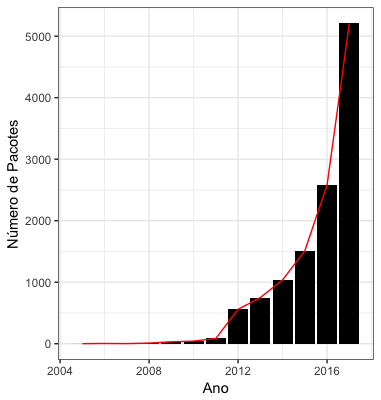
\includegraphics[width=0.8\textwidth]{./04-figuras/NRPackages}
	\fonte{\href{https://cran.r-project.org/web/packages/available_packages_by_date}
		{https://cran.r-project.org/web/packages/available\underline{ }packages\underline{ }by\underline{ }date}}
	\label{fig:RNPackages}
\end{figure}
